\documentclass{jsarticle}

\usepackage[dvipdfmx]{hyperref}
\usepackage[dvipdfmx,hiresbb]{graphicx}
\usepackage{float}
\usepackage{amsmath,amssymb}

\newcommand{\argmax}{\mathop{\rm arg~max}\limits}
\newcommand{\argmin}{\mathop{\rm arg~min}\limits}

\begin{document}

\title{ジョブショップスケジューリング}
\author{}

\maketitle

\section{問題設定}
n個の仕事(job)$J_1,\dots,J_n$をm台の機械(machine)$M_1,\dots,M_m$上で処理することを考える.
各仕事を処理する機械の順序は仕事ごとに予め与えられており,技術的順序(technological sequence)
と呼ばれる.
各機械$M_r$上での仕事$J_j$の処理のことを作業(operation)と呼び,$O_{j,r}$と表す.
各作業$O_{j,r}$は処理時間(processing time)$p_{j,r}$をかけて機械$M_r$上で中断なく処理される.
ここで各機械は全て異なり,同時に二つ以上の作業を処理することができないとする.
全ての仕事を完成させるまでの時間を総作業時間(makespan)と呼び$L$で表す.
この時,$n\times m$(総作業時間最小)一般ジョブショップスケジューリング問題
($n \times m$ \textit{minimum-makespan} general job-shop scheduling problem)(JSSP)とは,
各仕事の技術的順序と,各作業の処理時間が与えられて,$L$を最小にするような機械上での仕事の
処理順序を全て決定することである.

\section{スケジューリングの分類}
\begin{description}
	\item[ジョブショップスケジューリング] 
		製品を生産するのに必要な処理工程の順序が製品ごとに決まっている.
	\item[フローショップスケジューリング]
		全ての製品が同一な工程順序.
	\item[オープンショップスケジューリング]
		ジョブの一部,あるいは全部の工程順序が任意.
	\item[リエントラント性]
		同一の生産設備を2回以上使用する場合,リエントラント(re-entrant)性があるという.
		リエントラントジョブショップスケジューリング問題などという.
\end{description}

\begin{figure}[H]
	\centering
	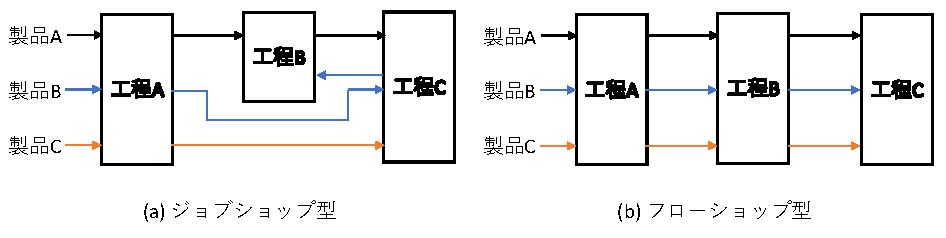
\includegraphics{figures/job_n_flow.pdf}
	\caption{スケジューリングの分類}
	\label{fig:job_n_flow}
\end{figure}

\section{背景技術}
\subsection{クリティカルブロック}
JSSPの解の表現方法として図~\ref{fig:disjunctive_graph}のような選択グラフ(disjunctive graph)
がよく用いられる
(※注:$O_{j,r}$の$r$は機械を表し,技術的順序ではないため,行列の要素とは対応しないことに注意).

\begin{figure}[H]
	\centering
	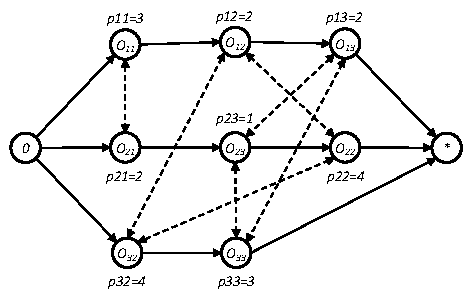
\includegraphics{figures/disjunctive_graph.pdf}
	\caption{選択グラフ}
	\label{fig:disjunctive_graph}
\end{figure}

JSSPは選択グラフ$G=(V,C\cup D)$を用いて次のように表現される.
\begin{itemize}
	\item Vは節点の集合であり,作業に対応する節点及び二つの特殊節点:ソース(0),シンク(*)からなる
	\item Cは節点間を結ぶ有向弧(conjunctive arc)の集合で,技術的順序を表す
	\item Dは選択弧(disjunctive arc)の集合で,同一機械上の作業の対を表す
\end{itemize}
各作業$O_{j,r}$の処理時間$p_{j,r}$は各節点に付与された重み$p_{j,i}$によって表す.
完全なスケジュールは同一機械上の全ての作業について処理順序を全て決定することによって得られる.
選択グラフモデルにおいて,このことは$D$の全ての無向(選択)弧を有向弧に変えることに対応する.
この時$D$より得られた有向弧の集合を「選択」(selection)$S$と呼ぶ.
ある選択$S$が実行可能スケジュールを表現していることと,有向グラフ$G(S)=(V,C\cup S)$が
サイクルを持たない(acyclic)こととは同値である.
この時$s$は「完全選択」(complete selection)と呼ばれる.
%対応するスケジュールの総作業時間は$0$から$*$に至る最も長い重みつきパスの長さによって与えられる.
%このパスはクリティカルパス$P$と呼ばれる.

各作業$O_{j,r}$の最遅完了時刻(Latest Finish Time)は,$O_{j,r}$の全ての後続作業の最遅完了時刻までに
到着するために,$O_{j,r}$を開始していなければいけない時刻である
(後続作業のLFTから自作業の処理時間を引いたものの最小値).
最早開始時刻(Earliest Start Time)と最遅完了時刻が等しい作業を結んだパスをクリティカルパス$P$と呼ぶ.

クリティカルパス上の作業列$B$は,次の性質が成り立つ時クリティカルブロック(または単にブロック)と
呼ばれる.
\begin{itemize}
	\item $B$の全ての作業は同一機械上にある
	\item $B$の最初(最後)の作業に先行(後続)する同一機械上の作業は(もし存在すれば)$P$上にない
\end{itemize}

\subsection{クリティカルブロック近傍}
一つの解$S$から一回の遷移によって到達可能な全ての解の集合を近傍$N(S)$と呼ぶ.
JSSPにおいて,例えばクリティカルブロック内の作業をそのブロッックの一番先頭,
もしくは最後へ移動させる遷移が用いられる.
この遷移を用いた近傍をクリティカルブロック近傍(CB近傍)と呼ぶ.
CB近傍$N^{C}(S)$を次のように定義する.

$B_j$をクリティカルパス$P$上,特定機械上の連続する作業$u_{i,j}$全体からなる,
j番目のブロックとする.すなわち$B_j=(u_{1,j},\dots,u_{i,j},\dots,u_{l_j,j})$,
ただし,$l_j$は$B_j$内の作業の個数である.
この時$P$は$(0,B_1,\dots,B_j,\dots,B_k,*)$のように表現される.
$l_j>1$なるブロック$B_j$に対して,次の二つの遷移操作$S^b$及び$S^a$を考える.
\begin{itemize}
	\item $S^b(S,u_{i,j})(1<i\leq l_j)$は,$S$のブロック$B_j$内の作業$u_{i,j}$を$B_j$の
		先頭に移動することによって得られる選択
	\item $S^a(S,u_{i,j})(1\leq i<l_j)$は,$S$のブロック$B_j$内の作業$u_{i,j}$を$B_j$の
		最後に移動することによって得られる選択
\end{itemize}
$S^b$もしくは$S^a$によって得られる選択はそれぞれ「前候補」(before candidate)もしくは
「後候補」(after candidate)と呼ばれる.
$S^b$及び$S^a$によって$S$より得られる全ての選択の集合は次のように表される.
\begin{equation}
	N^{'C}(S)=\left\{ S^b(S,u_{i,j})|l_j>1,i=2,\dots,l_j,j=1,\dots,k \right\}
	\left\{ S^a(S,u_{i,j})|l_j>1,i=1,\dots,l_j-1,j=1,\dots,k \right\}
\end{equation}
$N^{'C}(S)$の要素である選択の内のいくつかはサイクルを持つ可能性がある.
その場合対応するスケジュールは実行可能ではない.
したがって,クリティカルブロック近傍$N^C(S)$はそれらを除いて次のように与えられる.
\begin{equation}
	N^C(S)=\left\{S'\in N^{'C}(S)|S' は完全選択 \right\}
\end{equation}

仮に$S$が長さ2以上($l_j>1$)のブロックを一つも持たない場合$S$は最適解である.
なぜならこの時$P$の弧は全て$C$の元からなり,$L(S)$は$P$上の全作業の加工時間の和であり,
これは$L$の下界に等しい.
そうでない場合,$S$は少なくとも一つは長さ2以上のブロックを持ち,$N^{'C}(S)$は決して空ではない.
さらに$N^{'C}(S)$は実行可能でないスケジュールを含む可能性があるが,$N^C(S)$は決して空にならない.
なぜならブロック内の連続する二つの作業の処理順序の入れ替えによって決してサイクルは生じず,
したがって$S^b(S,u_{2,j})$及び$S^a(S,u_{l_j-1,j})$に対応する少なくとも二つの
スケジュールは常に実行可能である.

\subsection{GTアルゴリズム}
1つの完全選択から対応するスケジュールを生成する際,各作業を可能な限り早く加工して一意に得られる
スケジュールをセミアクティブスケジュールと呼ぶ.
セミアクティブスケジュールにおいて,ある作業の処理順序を,他の作業の処理開始時刻を遅らせることなく,
繰り上げて早められる場合がある(これをleft shiftと呼ぶ).
どの作業もこれ以上left shiftできないスケジュールをアクティブスケジュールと呼ぶ.
セミアクティブスケジュールのアクティブ化はしばしば解全体の改善につながる.
最適スケジュールは明らかにアクティブスケジュールであるので,探索空間を初めから
アクティブスケジュールに制限して最適化することで解法の効率化が期待できる.
アクティブスケジュールを生成するアルゴリズムとしては,
以下のGiffler and ThompsonのGTアルゴリズムが有名である.
\begin{enumerate}
	\item 技術的順序上,次に処理可能な作業の全体を$G$とし,$G$中,
		最早完了時刻が最も小さい作業を$O^*$とする.
		すなわち,$O^*=\argmin \left\{O\in G|EC(O) \right\}$.$O^*$を処理する機械を$M^*$とする.
		$M^*$が複数存在する場合,任意の一つを選択する.
	\item 機械$M^*$を利用する,最早開始時刻$ES(O)$が最早完了時刻$EC(O^*)$よりも小さい
		作業の集合(コンフリクト集合)$C[M^*,i]$を求める.
		ただし,$M^*$上すでにi-1個の作業が処理されているものとし,
		$C[M^*,i]= \left\{O\in G|ES(O)<EC(O^*) \right\}$.
	\item $M^*$上i番目に処理すべき作業を$C[M^*,i]$より一つ選び$O$とする.
	\item $O$の作業開始時刻を$ES(O)$と設定する
	\item 1に戻る($O^*$が空になれば終了)
\end{enumerate}

\subsubsection{例}
GTアルゴリズムによりアクティブスケジュールを生成する例を図~\ref{fig:GT}に示す.
ここで$T_E$は最早開始時刻(earliest node time)である.

\begin{itemize}
	\item (a)
	\begin{enumerate}
		\item $G=\left\{ O_{1,1},O_{2,1},O_{3,2} \right\}$ \\
			$EC(O_{1,1})=3, EC(O_{2,1})=2, EC(O_{3,2})=4 \therefore O^*=O_{2,1}, M^*=M_1$
		\item $ES(O_{1,1})=0, ES(O_{2,1})=0 \therefore C[M_1,1]=\left\{ O_{1,1}, O_{2,1} \right\}$
		\item $O=O_{1,1}$
	\end{enumerate}
	\item (b)
	\begin{enumerate}
		\item $G=\left\{ O_{1,2},O_{2,1},O_{3,2} \right\}$ \\
			$EC(O_{1,2})=5,EC(O_{2,1})=5,EC(O_{3,2})=4 \therefore
			O^*=\left\{ O_{1,2},O_{2,1} \right\} \rightarrow O_{1,2}, M^*=M_2$
		\item $ES(O_{1,2})=3,ES(O_{3,2})=0 \therefore C[M_2,1]=\left\{ O_{1,2},O_{3,2} \right\}$
		\item $O=O_{1,2}$
	\end{enumerate}
	\item (c)
	\begin{enumerate}
		\item $G=\left\{ O_{1,3},O_{2,1},O_{3,2} \right\}$ \\
			$EC(O_{1,3})=7,EC(O_{2,1})=5,EC(O_{3,2})=9 \therefore
			O^*=O_{2,1}, M^*=M_1$
		\item $ES(O_{2,1})=3 \therefore C[M_1,2]=\left\{ O_{2,1} \right\}$
		\item $O=O_{2,1}$
	\end{enumerate}
	\item (d)
	\begin{enumerate}
		\item $G=\left\{ O_{1,3},O_{2,3},O_{3,2} \right\}$ \\
			$EC(O_{1,3})=7,EC(O_{2,3})=6,EC(O_{3,2})=9 \therefore
			O^*=O_{2,3}, M^*=M_3$
		\item $ES(O_{1,3})=5,ES(O_{2,3})=5 \therefore C[M_3,1]=\left\{ O_{1,3},O_{2,3} \right\}$
		\item $O=O_{2,3}$
	\end{enumerate}
	\item (e)
	\begin{enumerate}
		\item $G=\left\{ O_{1,3},O_{2,2},O_{3,2} \right\}$ \\
			$EC(O_{1,3})=8,EC(O_{2,2})=10,EC(O_{3,2})=9 \therefore
			O^*=O_{1,3}, M^*=M_3$
		\item $ES(O_{1,3})=6 \therefore C[M_3,2]=\left\{ O_{1,3} \right\}$
		\item $O=O_{1,3}$
	\end{enumerate}
	\item (f)
	\begin{enumerate}
		\item $G=\left\{ O_{2,2},O_{3,2} \right\}$ \\
			$EC(O_{2,2})=10,EC(O_{3,2})=9 \therefore O^*=O_{3,2}, M^*=M_2$
		\item $ES(O_{2,2})=6,Es(O_{3,2})=5 \therefore C[M_2,2]=\left\{ O_{2,2},O_{3,2} \right\}$
		\item $O=O_{3,2}$
	\end{enumerate}
	\item (g)
	\begin{enumerate}
		\item $G=\left\{ O_{2,2},O_{3,3} \right\}$ \\
			$EC(O_{2,2})=13,EC(O_{3,3})=12 \therefore O^*=O_{3,3},M^*=M_3$
		\item $ES(O_{3,3})=9 \therefore C[M_3,3]=\left\{ O_{3,3} \right\}$
		\item $O=O_{3,3}$
	\end{enumerate}
\end{itemize}

\begin{figure}[H]
	\centering
	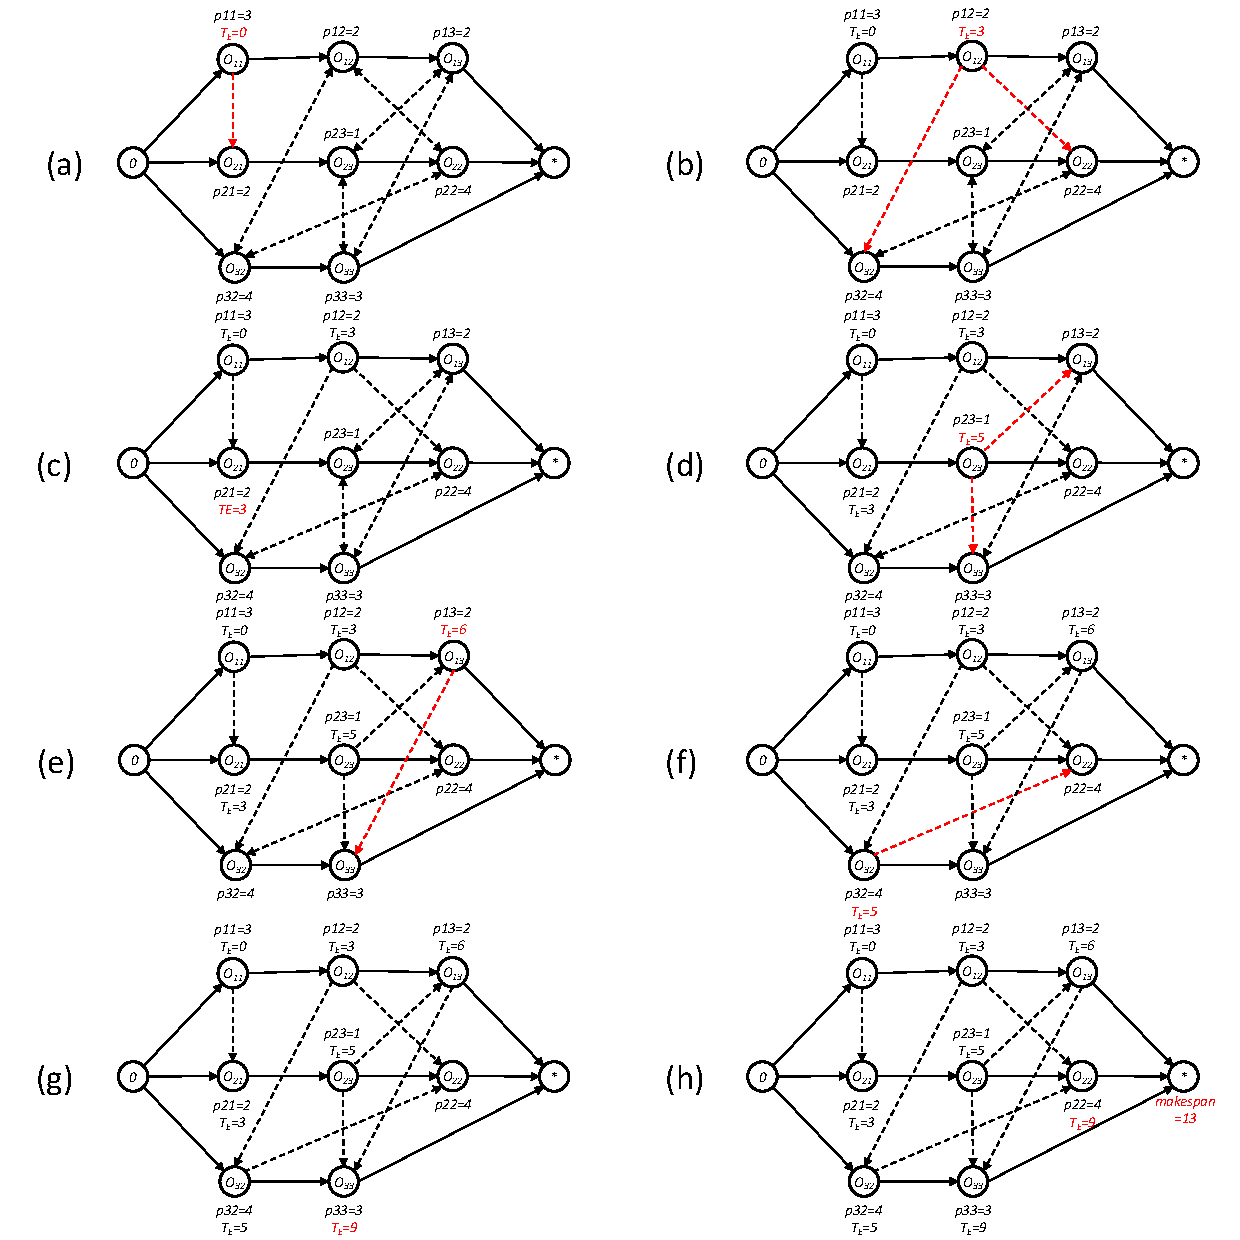
\includegraphics[scale=0.8]{figures/GT.pdf}
	\caption{GTアルゴリズムによるアクティブスケジュール生成例}
	\label{fig:GT}
\end{figure}


\begin{thebibliography}{9}
\bibitem{wakamiya1998}
  若宮 利治,片山 謙吾,成久 洋之,
  "スケジュール問題に対する有効な交叉法について",
  岡山理科大学紀要. A, 自然科学,
  vol. 34, pp. 307-318, 1998.

\bibitem{yamada1997}
  山田 武士,中野 良平,
  "遺伝的局所探索法によるジョブショップスケジューリング問題の解法",
  情報処理学会論文誌,
  vol. 38, no. 6, pp. 1126-1138, 1997.

\bibitem{moonen2004giffler}
  Moonen, M. and Janssens, G.K.,
  "A Giffler-Thompson Focused Genetic Algorithm for the Static Job-shop Scheduling Problem,"
  \textit{ITEO research paper series,}
  2004,

\bibitem{ripon2014}
  Kazi Shah Nawaz Ripon and Jim Torresen
  "Integrated job shop scheduling and layout planning: a hybrid evolutionary method for optimizing multiple objectives",
  \textit{Evolving Systems,}
  vol. 5, no. 2, pp. 121-132, 2014.

\bibitem{zalzala1997}
  Takeshi Yamada and Ryohei Nakano,
  "Chapter 7: Job-shop scheduling",
  \textit{Genetic Algorithms in Engineering Systems},
  pp. 134–-160, 1997.

\end{thebibliography}
\end{document}
